
\documentclass[]{article}
\voffset=-1.5cm
\oddsidemargin=0.0cm
\textwidth = 480pt

% http://www.strath.ac.uk/aer/materials/5furtherquantitativeresearchdesignandanalysis/unit6/whatislogisticregression/

% http://www.medcalc.org/manual/logistic_regression.php


\usepackage{amsmath}
\usepackage{graphicx}
\usepackage{amssymb}
\usepackage{framed}
\usepackage{multicol}
%\usepackage[paperwidth=21cm, paperheight=29.8cm]{geometry}
%\usepackage[angle=0,scale=1,color=black,hshift=-0.4cm,vshift=15cm]{background}
%\usepackage{multirow}
\usepackage{enumerate}





\begin{document}
	%%- https://statistics.laerd.com/statistical-guides/dependent-t-test-statistical-guide.php
	
	\section*{Lab 2 Part D: Dependent t-test for paired samples}
	
\section{Introduction}
	The dependent t-test (also called the paired t-test or paired-samples t-test) compares the means of \textbf{\textit{two related groups}} to determine whether there is a statistically significant difference between these means.
	
\subsection{What variables do you need for a dependent t-test?}
	You need one dependent variable that is measured on an interval or ratio scale. You also need one categorical variable that has only two related groups.
	
	%===============================================================%
	\subsection{What is meant by ``related groups" or ``paired groups"?}
\begin{itemize}
\item A dependent t-test is an example of a ``within-subjects" or ``repeated-measures" statistical test. 
\item This indicates that the same participants are tested more than once. Thus, in the dependent t-test, ``related groups" indicates that the same participants are present in both groups. 
\item The reason that it is possible to have the same participants in each group is because each participant has been measured on two occasions on the same dependent variable. 
\item For example, you might have measured the performance of 10 participants in a spelling test (the dependent variable) before and after they underwent a new form of computerised teaching method to improve spelling. 
\item You would like to know if the computer training improved their spelling performance. Here, we can use a dependent t-test because we have two related groups. 
\item The first related group consists of the participants at the beginning (prior to) the computerised spell training and the second related group consists of the same participants, but now at the end of the computerised training.
\end{itemize}
	
	
	%==============================================================================%
	\newpage
	\subsection*{Introduction}
\begin{itemize}
	\item 	The dependent t-test (called the paired-samples t-test in SPSS Statistics) compares the means between two related groups on the same continuous, dependent variable. For example, you could use a dependent t-test to understand whether there was a difference in smokers' daily cigarette consumption before and after a 6 week hypnotherapy programme (i.e., your dependent variable would be ``daily cigarette consumption", and your two related groups would be the cigarette consumption values "before" and "after" the hypnotherapy programme). If your dependent variable is dichotomous, you should instead use McNemar's test.
	
\item This guide shows you how to carry out a dependent t-test using SPSS Statistics, as well as interpret and report the results from this test. However, before we introduce you to this procedure, you need to understand the different assumptions that your data must meet in order for a dependent t-test to give you a valid result. We discuss these assumptions next.
\end{itemize}

	

\section{Sport Science Student Exercise - Example}
\begin{itemize}
	\item A group of Sports Science students (n = 20) are selected from the population to investigate whether a 12-week plyometric-training programme improves their standing long jump performance.
	\item  In order to test whether this training improves performance, the students are tested for their long jump performance before they undertake a plyometric-training programme and then again at the end of the programme (i.e., the dependent variable is "\textbf{\textit{standing long jump performance}}", and the two related groups are the standing long jump values ``before" and ``after" the 12-week plyometric-training programme).
	
\end{itemize}

\newpage	
\subsection{Test Procedure in SPSS Statistics}
	The six steps below show you how to analyse your data using a dependent t-test in SPSS Statistics when the four assumptions in the previous section, Assumptions, have not been violated. 
	
	At the end of these six steps, we show you how to interpret the results from this test. 

%% If you are looking for help to make sure your data meets assumptions No. 3 and No. 4, which are required when using a dependent t-test, and can be tested using SPSS Statistics, you can learn more in our enhanced guides here. 
	
%	We also show you how to correctly enter your data into SPSS Statistics in order to run a dependent t-test, as well as explaining how to deal with missing values (e.g., if a participant completed a pre-test but failed to turn up to the post-test). However, in this "quick start" guide, we focus on the six steps required to run the dependent t-test procedure using SPSS Statistics.
	
\noindent Click \textbf{Analyze $>$ Compare Means $>$ Paired-Samples T Test}... on the top menu, as shown below:
	
\begin{figure}[h!]
\centering
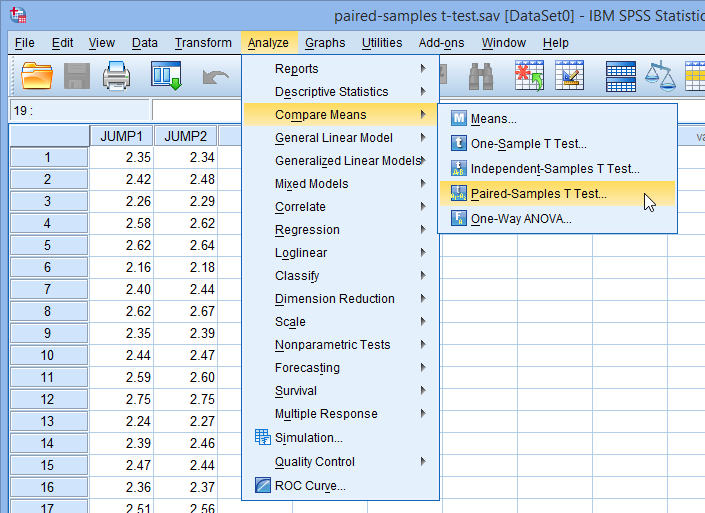
\includegraphics[width=0.5\linewidth]{Paired/pairedMenu1}

\label{fig:pairedMenu1}
\end{figure}

	You will be presented with the Paired-Samples T Test dialogue box, as shown below:
	
\begin{figure}[h!]
	\centering
	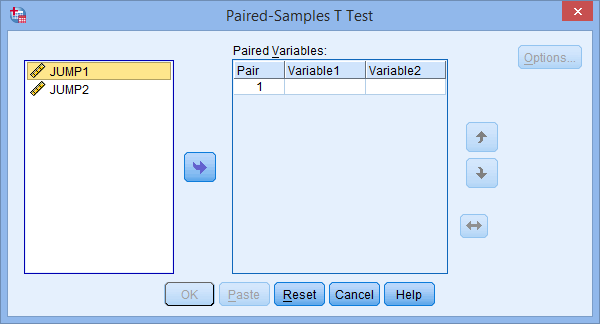
\includegraphics[width=0.5\linewidth]{Paired/pairedMenu2}

	\label{fig:pairedMenu2}
\end{figure}

\noindent Transfer the variables JUMP1 and JUMP2 into the \texttt{Paired Variables:} box. There are two ways to do this:
\begin{itemize}
	\item[(a)] click on both variables whilst holding down the shift key (which highlights them) and then pressing the SPSS Right Arrow Button button; 
	\item[(b)] drag-and-drop each variable separately into the boxes. 
\end{itemize}	
 
\begin{framed}	
\noindent \textit{If you are using older versions of SPSS Statistics, you will need to transfer the variables using the former method. You will end up with a screen similar to the one shown below:}
\end{framed}	
\begin{figure}[h!]
	\centering
	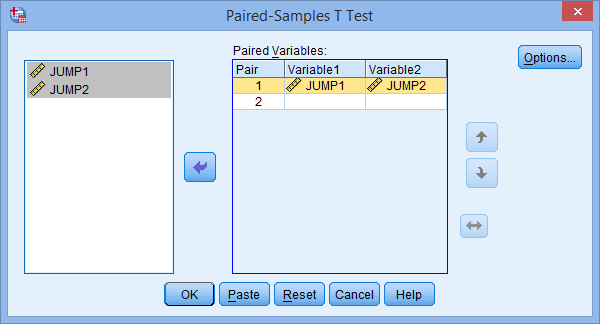
\includegraphics[width=0.5\linewidth]{Paired/pairedMenu3}

	\label{fig:pairedMenu3}
\end{figure}

\begin{figure}
\centering
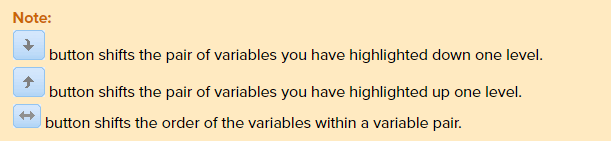
\includegraphics[width=0.6\linewidth]{Paired/Buttons}

\label{fig:Buttons}
\end{figure}

	
	If you need to change the confidence level limits or exclude cases, click on the Options Button button. You will be presented with the Paired-Samples T Test: Options dialogue box, as shown below:
	
\begin{figure}[h!]
	\centering
	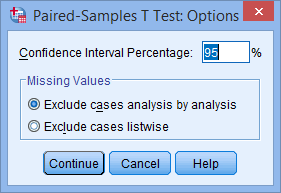
\includegraphics[width=0.5\linewidth]{Paired/pairedMenu4}

	\label{fig:pairedMenu4}
\end{figure}
	Click the \texttt{Continue} button. You will be returned to the Paired-Samples T Test dialogue box. Then click the \texttt{OK} button.
	
	%===================================================================================%
\newpage
\subsection{Output of the Dependent T-Test in SPSS Statistics}
\begin{itemize}
	\item SPSS Statistics generates three tables in the Output Viewer under the title "T-Test", but you only need to look at two tables: \textbf{the Paired Samples Statistics table} and the \textbf{Paired Samples Test table}.\smallskip
	\item In addition, you will need to interpret the boxplots that you created to check for outliers and the output from the Shapiro-Wilk test for normality, which you used to determine whether the distribution of the differences in the dependent variable between the two related groups were approximately normally distributed. \smallskip
%	\item This is explained in our enhanced guide. However, in this "quick start" guide, we focus on the two main tables you need to understand if your data has met all the necessary assumptions:
\end{itemize}

	


	The first table, titled Paired Samples Statistics, is where SPSS Statistics has generated descriptive statistics for your variables. You could use the results here to describe the characteristics of the first and second jumps in your write-up.
	
\begin{figure}[h!]
\centering
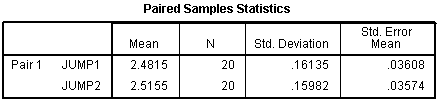
\includegraphics[width=0.7\linewidth]{Paired/PairedOutput1}

\label{fig:PairedOutput1}
\end{figure}

	
\subsection{Paired Samples Test Table}
	The Paired Samples Test table is where the results of the dependent t-test are presented. A lot of information is presented here and it is important to remember that this information refers to the differences between the two jumps (the subtitle reads "Paired Differences"). As such, the columns of the table labelled "Mean", "Std. Deviation", "Std. Error Mean" and "95\% Confidence Interval of the Difference" refer to the mean difference between the two jumps and the standard deviation, standard error and 95\% confidence interval of this mean difference, respectively. 
	
	The last three columns express the results of the dependent t-test, namely the t-value ("t"), the degrees of freedom ("df") and the significance level ("Sig. (2-tailed)").
	
\begin{figure}[h!]
	\centering
	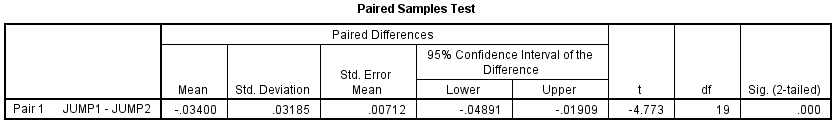
\includegraphics[width=0.7\linewidth]{Paired/PairedOutput2}
	\caption{}
	\label{fig:PairedOutput2}
\end{figure}

	You are essentially conducting a one-sample t-test on the differences between the groups.
	
\newpage	
%=============================================================%
\section{Reporting the Output of the Dependent T-Test}
	You might report the statistics in the following format: t(degrees of freedom) = t-value, p = significance level. In our case this would be: t(19) = -4.773, p < 0.0005. Due to the means of the two jumps and the direction of the t-value, we can conclude that there was a statistically significant improvement in jump distance following the plyometric-training programme from 2.48 ± 0.16 m to 2.52 ± 0.16 m (p < 0.0005); an improvement of 0.03 ± 0.03 m.
	
	\begin{framed}
	\textit{
	Note: SPSS Statistics can output the results to many decimal places, but you should understand your measurement scale in order to know whether it is appropriate to report your results with such precision.}
	\end{framed}
%	\begin{itemize}
%		\item In our enhanced dependent t-test guide, we show you how to write up the results from your assumptions tests and dependent t-test procedure if you need to report this in a dissertation/thesis, assignment or research report. 
%		\item We do this using the Harvard and APA styles. It is also worth noting that in addition to reporting the results from your assumptions and dependent t-test, you are increasingly expected to report effect sizes. 
%		\item Whilst there are many different ways you can do this, we show you how to calculate effect sizes from your SPSS Statistics results in our enhanced dependent t-test guide. Effect sizes are important because whilst the dependent t-test tells you whether differences between group means are "real" (i.e., different in the population), it does not tell you the "size" of the difference. Providing the effect size in your results helps to overcome this limitation. You can learn more about our enhanced content here.
%	\end{itemize}
	
	
\section*{Assumptions}
\begin{itemize}
	\item 	When you choose to analyse your data using a dependent t-test, part of the process involves checking to make sure that the data you want to analyse can actually be analysed using a dependent t-test. 
	
	\item You need to do this because it is only appropriate to use a dependent t-test if your data ``passes" four assumptions that are required for a dependent t-test to give you a valid result. 
	
	
	\item In practice, checking for these four assumptions just adds a little bit more time to your analysis, requiring you to click a few more buttons in SPSS Statistics when performing your analysis, as well as think a little bit more about your data, but it is not a difficult task.
	
	\item Before we introduce you to these four assumptions, do not be surprised if, when analysing your own data using SPSS Statistics, one or more of these assumptions is violated (i.e., is not met). 
	
	\item This is not uncommon when working with real-world data rather than textbook examples, which often only show you how to carry out a dependent t-test when everything goes well! However, don't worry. Even when your data fails certain assumptions, there is often a solution to overcome this.
	
\end{itemize}


First, let's take a look at these four assumptions:

\begin{description}
	\item[ Assumption No. 1:] Your dependent variable should be measured on a continuous scale (i.e., it is measured at the interval or ratio level). Examples of variables that meet this criterion include revision time (measured in hours), intelligence (measured using IQ score), exam performance (measured from 0 to 100), weight (measured in kg), and so forth. You can learn more about continuous variables in our article: Types of Variable.
	\item[ Assumption No. 2:] Your independent variable should consist of two categorical, "related groups" or "matched pairs". "Related groups" indicates that the same subjects are present in both groups. The reason that it is possible to have the same subjects in each group is because each subject has been measured on two occasions on the same dependent variable. For example, you might have measured 10 individuals' performance in a spelling test (the dependent variable) before and after they underwent a new form of computerised teaching method to improve spelling. You would like to know if the computer training improved their spelling performance. 
	
	The first related group consists of the subjects at the beginning of (prior to) the computerised spelling training and the second related group consists of the same subjects, but now at the end of the computerised training. The dependent t-test can also be used to compare different subjects, but this does not happen very often.
	%% Nonetheless, to learn more about the different study designs that can be analysed using a dependent t-test, see our enhanced dependent t-test guide.
	\item[ Assumption No. 3:] There should be no significant outliers in the differences between the two related groups. Outliers are simply single data points within your data that do not follow the usual pattern (e.g., in a study of 100 students' IQ scores, where the mean score was 108 with only a small variation between students, one student had a score of 156, which is very unusual, and may even put her in the top 1\% of IQ scores globally). The problem with outliers is that they can have a negative effect on the dependent t-test, reducing the validity of your results. In addition, they can affect the statistical significance of the test. Fortunately, when using SPSS Statistics to run a dependent t-test on your data, you can easily detect possible outliers. 
	%%In our enhanced dependent t-test guide, we (a) show you how to use SPSS Statistics to compute the difference scores, (b) show you how to detect outliers using SPSS Statistics, and (c) discuss some of the options you have in order to deal with outliers.
	\item[ Assumption No. 4:] The distribution of the differences in the dependent variable between the two related groups should be approximately normally distributed. We talk about the dependent t-test only requiring approximately normal data because it is quite "robust" to violations of normality, meaning that the assumption can be a little violated and still provide valid results. You can test for normality using the Shapiro-Wilk test of normality, which is easily tested for using SPSS Statistics.
	%% In addition to showing you how to do this in our enhanced dependent t-test guide, we also explain what you can do if your data fails this assumption (i.e., if it fails it more than a little bit).
\end{description}
\subsection*{Checking Assumptions}	
\begin{itemize}
	\item You can check assumptions No. 3 and No. 4 using SPSS Statistics. Before doing this, you should make sure that your data meets assumptions No. 1 and No. 2, although you don't need SPSS Statistics to do this. When moving on to assumptions No. 3 and No. 4, we suggest testing them in this order because it represents an order where, if a violation to the assumption is not correctable, you will no longer be able to use a dependent t-test (although you may be able to run another statistical test on your data instead). 
	
	\item Just remember that if you do not run the statistical tests on these assumptions correctly, the results you get when running a dependent t-test might not be valid. 
	%%This is why we dedicate a number of sections of our enhanced dependent t-test guide to help you get this right. You can find out about our enhanced content as a whole here, or more specifically, learn how we help with testing assumptions here.
	
	\item In the section, Test Procedure in SPSS Statistics, we illustrate the SPSS Statistics procedure required to perform a dependent t-test assuming that no assumptions have been violated. First, we set out the example we use to explain the dependent t-test procedure in SPSS Statistics.
\end{itemize}


%===================================================================================%

\end{document}